\documentclass[UTF8]{ctexart}
% 基本设置和必要宏包
\usepackage{geometry}
\geometry{a4paper,scale=0.8}

% 数学相关宏包
\usepackage{amsmath}
\usepackage{amssymb}
\usepackage{amsfonts}

\usepackage{mathtools}
\usepackage{amsbsy}
\usepackage{amstext}
\usepackage{wasysym}
\usepackage{stmaryrd}
\usepackage{mathrsfs}

% 图形和颜色
%\usepackage{xcolor}
\usepackage{graphicx}
\usepackage{subcaption}
\usepackage{caption}
\usepackage{float}



% 其他功能性宏包
\usepackage{titlesec}
\usepackage{fancyhdr}
\usepackage{setspace}
\usepackage{cite}
\usepackage{appendix}
\usepackage{listings}
\usepackage{pdfpages}
\usepackage{enumitem}
\usepackage{tabu}
\usepackage{threeparttable}
\usepackage{booktabs}
\usepackage{abstract}


\usepackage{diagbox} 
% 设置全局字体
%\setCJKmainfont{SimSun} % 设置正文为宋体
%\setCJKsansfont{SimHei} % 设置无衬线字体为黑体

% 允许公式跨页
\allowdisplaybreaks[4]



\newcommand{\sihaoheiti}{\fontsize{14pt}\selectfont\heiti}

% 论文题目设置为三号黑体字,并居中
\newcommand{\threelargebf}{\fontsize{16pt}{19.2pt}\selectfont\heiti\centering}

% 一级标题设置为四号黑体字,并居中
\titleformat{\section}{\centering\fontsize{14pt}{16pt}\bfseries\heiti}{\thesection}{1em}{}

% 二级标题设置为小四号黑体字,左对齐
\titleformat{\subsection}{\fontsize{12pt}{14.4pt}\bfseries\heiti}{\thesubsection}{1em}{\raggedright}

% 三级标题设置为小四号黑体字,左对齐
\titleformat{\subsubsection}{\fontsize{12pt}{14.4pt}\bfseries\heiti}{\thesubsubsection}{1em}{\raggedright}

% 正文字体设置为小四号宋体字,并使用单倍行距
\renewcommand{\normalsize}{\fontsize{12pt}{14.4pt}\selectfont}


%\linespread{5.0}% 修改行距

%图片文件夹
\graphicspath{{img/}}

\let\itemize\compactitem
\let\enditemize\endcompactitem

% 设置页面布局
\geometry{a4paper, left=2.5cm, right=2.5cm, top=3cm, bottom=3cm}
\setstretch{1.2}

\renewcommand{\arraystretch}{1.5}
\newcommand{\thickhline}{\noalign{\hrule height 1.2pt}} % 设置粗线的宽度
\newcommand{\thinhline}{\noalign{\hrule height 0.8pt}} % 设置细线的宽度

%%%% ===== 定理环境
\usepackage[amsmath,thref,thmmarks,hyperref]{ntheorem} % 定理宏包
%\theorempreskipamount1em % spacing before the environment
%\theorempostskipamount0em  % spacing after the environment
%\theoremstyle{plain}
%\theoremheaderfont{\normalfont\heiti}
%\theorembodyfont{\normalfont\kaishu}
%\theoremindent0em
%\theoremseparator{\hspace{0.2em}}
%\theoremnumbering{arabic}

\newtheorem{property}{性质}[section]
\newtheorem{definition}{定义}[section]
\newtheorem{lemma}{引理}[section]
\newtheorem{remark}{注记}[section]
\newtheorem{corollary}{推论}[section]
\newtheorem{example}{例}[section] 
\newtheorem{problem}{{问题}}

\renewcommand{\abstractnamefont}{\normalfont\bfseries}  % 摘要标题字体:正常字体,粗体
\renewcommand{\abstracttextfont}{\normalfont\normalsize}     % 摘要内容字体:正常字体,小四号

% 设置页眉页脚
\pagestyle{fancy}
\fancyhf{}
\fancyfoot[C]{\thepage}
\renewcommand{\headrulewidth}{0pt}

% 设置标题格式
\titleformat{\section}{\centering\heiti\large}{\thesection}{1em}{}
\titleformat{\subsection}{\raggedright\heiti\normalsize}{\thesubsection}{1em}{}
\titleformat{\subsubsection}{\raggedright\heiti\normalsize}{\thesubsubsection}{1em}{}

% 设置摘要环境
%\newenvironment{myabstract}{
%	\begin{center}
%	\bfseries\zihao{-3} 摘要
%	\end{center}
%	\vspace{-0.5em} % 调整摘要与论文题目的距离
%	\normalsize
%}{
%}
% 设置附录环境
\renewcommand{\appendixname}{附录}
\renewcommand{\appendixpagename}{附录}

% 设置代码环境
\lstset{
	basicstyle=\small\ttfamily,
	keywordstyle=\color{blue},
	commentstyle=\color{green!70!black},
	stringstyle=\color{red},
	breaklines=true,
	numbers=left,
	numberstyle=\tiny,
	frame=tb,
	language=Python
}
\newcommand{\bbA}{\mathbb{A}}
\newcommand{\bbB}{\mathbb{B}}
\newcommand{\bbC}{\mathbb{C}}
\newcommand{\bbD}{\mathbb{D}}
\newcommand{\bbE}{\mathbb{E}}
\newcommand{\bbF}{\mathbb{F}}
\newcommand{\bbG}{\mathbb{G}}
\newcommand{\bbH}{\mathbb{H}}
\newcommand{\bbI}{\mathbb{I}}
\newcommand{\bbJ}{\mathbb{J}}
\newcommand{\bbK}{\mathbb{K}}
\newcommand{\bbL}{\mathbb{L}}
\newcommand{\bbM}{\mathbb{M}}
\newcommand{\bbN}{\mathbb{N}}
\newcommand{\bbO}{\mathbb{O}}
\newcommand{\bbP}{\mathbb{P}}
\newcommand{\bbQ}{\mathbb{Q}}
\newcommand{\bbR}{\mathbb{R}}
\newcommand{\bbS}{\mathbb{S}}
\newcommand{\bbT}{\mathbb{T}}
\newcommand{\bbU}{\mathbb{U}}
\newcommand{\bbV}{\mathbb{V}}
\newcommand{\bbW}{\mathbb{W}}
\newcommand{\bbX}{\mathbb{X}}
\newcommand{\bbY}{\mathbb{Y}}
\newcommand{\bbZ}{\mathbb{Z}}

\title{}
\author{}
\date{}

\begin{document}
\begin{titlepage}		
		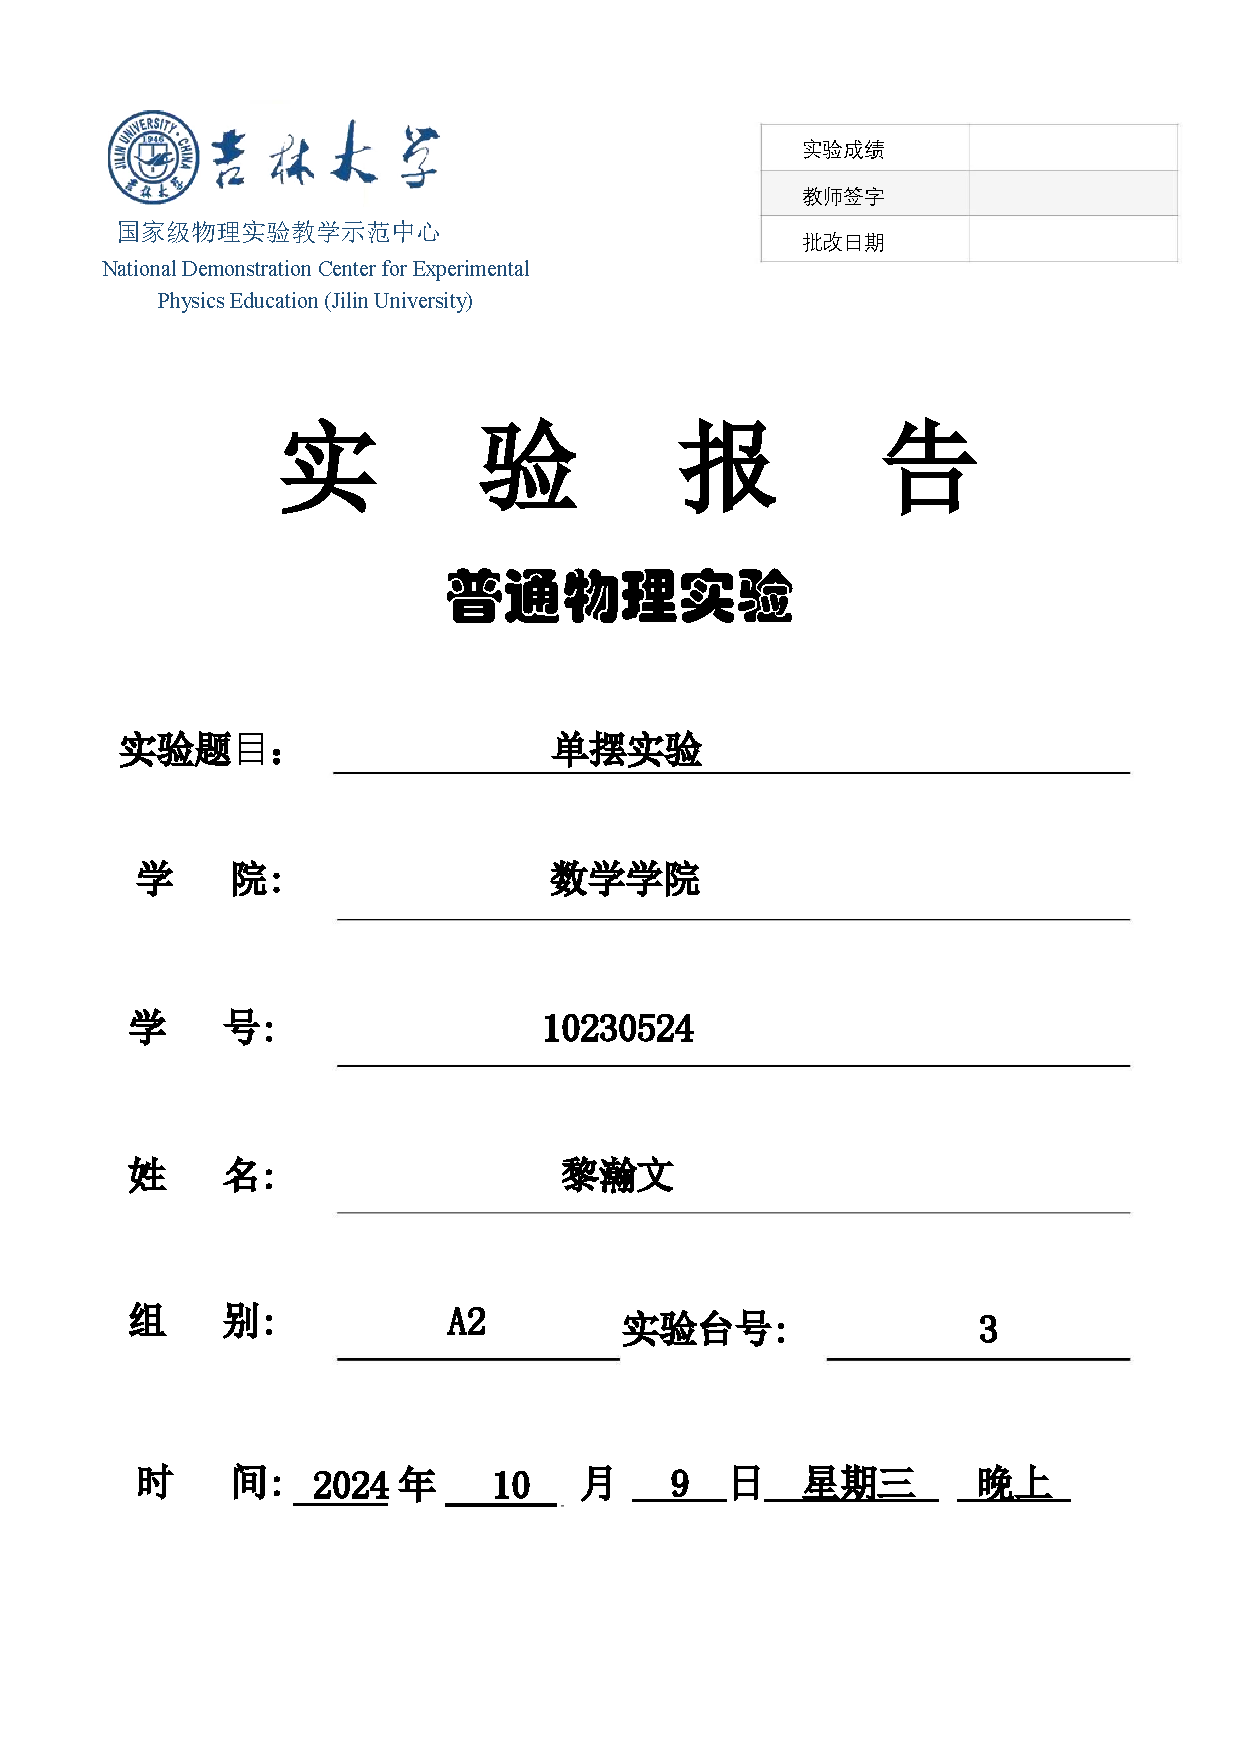
\includepdf[pages=-]{单摆封面.pdf}
\end{titlepage}

\section{实验内容}
\begin{enumerate}
    \item 调节单摆支架底脚螺丝,使摆线垂直于地面
    \item 将悬线一端固定在摆球上,另一端固定在支架上读出从悬点到乒乓球底端的距离$l$ 
    \item 摆长固定为 $60cm$,将乒乓球拉离平衡位置,使悬线与竖直方向成一适当小的角度 $\theta$,用数字毫伏计测量乒乓球摆动5个周期所需的时间,测量5次
    \item 改变摆长分别为 $70cm$、$80cm$、$90cm$、$95cm$(摆长$95cm$是由于实验中悬线长度不足$100cm$ 故取悬线最大值)
    \item 测量摆角仪大小,据此将摆角仪调至能读角度位置
    \item 固定摆长为 $90cm$,改变摆角分别为 $10^{\circ}$、$15^{\circ}$、$20^{\circ}$、$25^{\circ}$、$30^{\circ}$ 

\end{enumerate}
\section{原始数据}


\begin{table}[H]
\centering
\caption{测量乒乓球直径}
\begin{tabular}{|c|c|c|c|c|c|}
\toprule[1pt]
直径D/mm & 25.02 & 25.00 & 25.02 & 25.00 & 25.00 \\
\bottomrule[1pt]
\end{tabular}
\end{table}

\begin{table}[H]
\centering
\caption{测量 $ \theta = 10^{\circ}$ 时不同摆长的单摆运动5个周期的时间}
\begin{tabular}{|c|c|c|c|c|c|}
\toprule[1pt]
\midrule
摆长$l/cm$ & 1 & 2 & 3 & 4 & 5 \\
\midrule
60 & 7.5853 & 7.5848 & 7.5860 & 7.5858 & 7.5847 \\
\midrule
70 & 8.2086 & 8.2086 & 8.2083 & 8.2089 & 8.2080 \\
\midrule
80 & 8.7849 & 8.7851 & 8.7844 & 8.7843 & 8.7854 \\
\midrule
90 & 9.3451 & 9.3455 & 9.3450 & 9.3455 & 9.3446 \\
\midrule
95 & 9.6322 & 9.6319 & 9.6326 & 9.6322 & 9.6326 \\
\midrule
\bottomrule[1pt]
\end{tabular}
\begin{tablenotes}
\centering
    \footnotesize
    \item[*] *运动时间单位为 $s$
\end{tablenotes}

\end{table}


\begin{table}[H]

\centering
\caption{摆长为 $90cm$ 时不同 $\theta$ 运动5个周期的时间}
\begin{tabular}{|c|c|c|c|c|c|}
\toprule[1pt]
\midrule
摆角$\theta /^{\circ}$ & 1 & 2 & 3 & 4 & 5 \\
\midrule
10 & 9.3456 & 9.3460 & 9.3457 & 9.3464 & 9.3464 \\
\midrule
15 & 9.3682 & 9.3688 & 9.3690 & 9.3677 & 9.3685 \\
\midrule
20 & 9.3978 & 9.3999 & 9.3997 & 9.3989 & 9.3992 \\
\midrule
25 & 9.4351 & 9.4377 & 9.4361 & 9.4361 & 9.4375 \\
\midrule
30 & 9.4811 & 9.4803 & 9.4809 & 9.4817 & 9.4811 \\
\midrule
\bottomrule[1pt]
\end{tabular}
\begin{tablenotes}
\centering
    \footnotesize
    \item[*] *运动时间单位为 $s$
\end{tablenotes}

\end{table}

计算原始数据中经过5次测量得到的数据的平均值为
\begin{table}[H]
\centering
\caption{原始数据得到测量时间的平均值}
\begin{tabular}{|c|c|c|c|c|c|}
\toprule[1pt]
\midrule
摆长$l/cm$ & 60 & 70 & 80 & 90 & 95 \\
\midrule
$\overline{T} /s$ & 7.58532& 8.20848& 8.78482 & 9.34514& 9.63230 \\
\midrule
 摆角$\theta /^{\circ}$ & 10 & 15 & 20 & 25 & 30 \\
\midrule
$\overline{T} /s$ & 9.34602& 9.36844 & 9.3991 & 9.43650 & 9.48102 \\
 \midrule
\bottomrule[1pt]
\end{tabular}
\end{table}




\section{数据处理与分析}
\subsection{数据处理分析问题一}
\subsubsection{数据处理、绘图与计算斜率、求重力加速度$g$}



\begin{figure}[H]  %h此处,t页顶,b页底,p独立一页,浮动体出现的位置
		\centering
		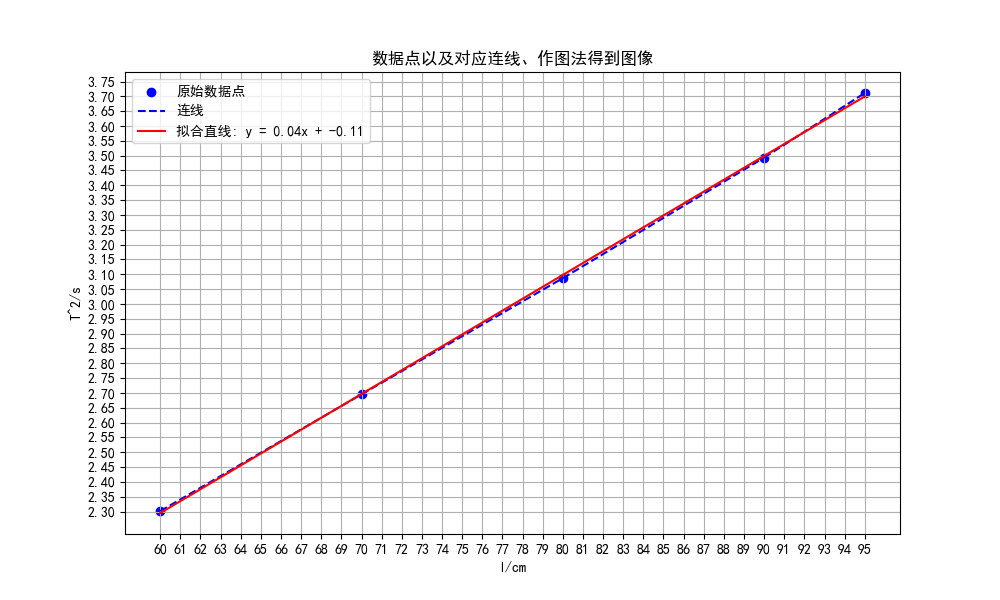
\includegraphics[width=0.8\textwidth,height=0.5\textwidth]{img/单摆周期平方作图法图像.png}
		%\caption{}
		\label{fig:side:b} 
\end{figure}

通过计算机模拟作图法得到图像如图所示
其中由于上述测得数据为单摆运动5个周期所得到的数据,故经过计算一个周期内以$T^2$为纵坐标、$l$为横坐标得到的直线的的斜率 $k = 0.0401319 \  s^2/cm$

通过单位代换得到 $k = 4.01319 \ s^2/m$,
由公式
\begin{align*}
    T^2 = \frac{4\pi^2 l}{g}
\end{align*}
 
 带入 $k = 4.01319 \ s^2/m$ 得到 
\begin{align*}
    g = \frac{4 \pi^2 }{k} = \frac{4 \pi^2}{4.01319} m/s^2 = 9.83717 m/s^2
\end{align*}
 求得重力加速度为 $9.83717 m/s^2$

\subsubsection{与实际值比较并计算百分差}
查询数据得到长春当地重力加速度为 $g_{\text{理论}} = 9.80476 m/s^2$。显然计算得到的 重力加速度比理论值更大。由百分差计算公式
\begin{align*}
    \alpha &= \frac{g - g_{\text{理论}}}{g_{\text{理论}}} \times 100 \% \\ 
    &= \frac{9.83717 - 9.80476}{9.80476} \times 100 \% = 0.3306 \% 
\end{align*}

得到百分差为 $0.3306 \%$

\subsection{数据处理分析问题二}
\subsubsection{根据作图法不确定度计算方法,计算斜率 $k$ 的扩展不确定度}
测量数据时,测量单摆仪器上的分度值为 $ \Delta x = 0.1cm$,作图法中 $T^2$ 的分度值为 $\Delta y = 0.05s^2$。设误差概率密度满足均匀分布,则其标准不确定度

\begin{align*}
    u(T^2) &= \frac{\Delta y}{\sqrt{3}}  = \frac{0.05}{\sqrt{3}} s^2 = 0.028867 s^2 \\
    u(l) &= \frac{\Delta x}{\sqrt{3}} = \frac{0.1}{\sqrt{3}} cm = 0.057735 cm 
\end{align*}

由作图法得到的直线上两点坐标设为 $(x_1,y_1)$,$(x_2,y_2)$,得到斜率为
\begin{align*}
    k = \frac{y_2 - y_1}{x_2 - x_1}
\end{align*}
取对数得到
\begin{align*}
    \ln{k} = \ln{(y_2 - y_1)} - \ln{(x_2 - x_1)}
\end{align*}
利用相对不确定度传递公式得
\begin{align*}
    \frac{u_k}{|k|} &= \sqrt{ 
    \Big(   \frac{\partial \ln{k} }{\partial y_2}        \Big)^2u^2(y_2)     +
    \Big(   \frac{\partial \ln{k} }{\partial y_1}        \Big)^2u^2(y_1)     +
    \Big(   \frac{\partial \ln{k} }{\partial x_2}        \Big)^2u^2(x_2)     +
    \Big(   \frac{\partial \ln{k} }{\partial x_1}        \Big)^2u^2(x_1)  
    } \\
    &= \sqrt{ 
    \Big(   \frac{1 }{y_2 - y_1}        \Big)^2u^2(y_2)     +
    \Big(   \frac{-1 }{y_2 - y_1}        \Big)^2u^2(y_1)     +
    \Big(   \frac{-1 }{x_2 - x_1}        \Big)^2u^2(x_2)     +
    \Big(   \frac{1 }{x_2 - x_1}        \Big)^2u^2(x_1)  
    }
\end{align*}

取曲线上两点得 $\frac{u_k}{|k|} =  0.051026  $,带入 $k = 4.01319 \ s^2/m $得到 $u_k = 0.20478 \ s^2/m $

扩展不确定度 取置信概率 $p = 0.955$,$K_p = 2$,则 $j=k$ 的扩展不确定度$U_k$为:
\begin{align*}
    U_k = K_p u_k = 2 \times 0.20478 \ s^2/m = 0.40956 \ s^2/m
\end{align*}

$k = 4.01319 \pm 0.40956 \  s^2/m $







\subsubsection{计算重力加速度 $g$ 的扩展不确定度}
已知公式
\begin{align*}
    g &= \frac{4\pi l}{T^2} \\
\end{align*}
由不确定度传递公式
\begin{align*}
    u(L) = \sqrt{\sum (\frac{\partial L}{\partial x_i})^2u(x_i)^2 } 
\end{align*}
经计算得
\begin{align*}
    \frac{u_g}{g} &= \sqrt{
    \frac{u^2(l)}{\overline{l}^2} +
    \frac{u^2(T^2)}{(\overline{T^2})^2}
    }    \\
    &= \sqrt{\frac{0.057735^2}{79^2} +
    \frac{0.028867^2}{3.03541^2}
    } = 0.00953812 
\end{align*}
经计算可得到 $u_g = 0.0938281 m/s^2$

扩展不确定度 取置信概率 $p = 0.955$,$K_p = 2$,则$U_g$:
\begin{align*}
    U_g = K_p u_g  = 2 \times 0.0938281 \ m/s^2 = 0.1876562 \ m/s^2
\end{align*}
故综上所述 $g = 9.83717 \pm 0.18766 \ m/s^2$

\subsection{用最小二乘法验证单摆周期与摆角关系}
 \begin{figure}[H]  %h此处,t页顶,b页底,p独立一页,浮动体出现的位置
		\centering
		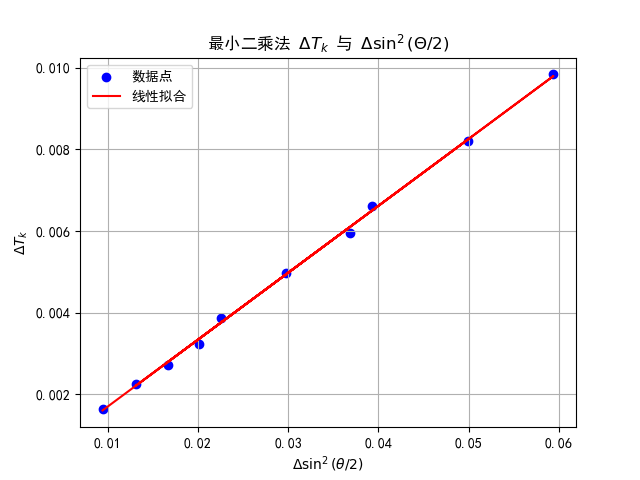
\includegraphics[width=0.8\textwidth,height=0.6\textwidth]{img/周期差与sin差.png}
		%\caption{}
		\label{fig:side:b} 
\end{figure}
最小二乘法拟合得到的直线 $y = ax+b$ 的斜率 $a$ 为 $0.164148$,一次项为 $0.00004997$ 

结合图像和最小二乘法拟合系数可看出:任取两组 $T_k$、$T_i$,记$T_k - T_i = \Delta T$、$\sin^2(\frac{\theta_k}{2}) - \sin^2(\frac{\theta_i}{2})= \Delta \sin^2(\frac{\theta}{2})$,显然 $\Delta T$ 与 $ \Delta \sin^2(\frac{\theta}{2})$ 成正比关系,比值为常数 $a = 0.164148$



\section{思考题}
\subsection{空气阻尼是否影响单摆周期}
在理想情况下,没有空气阻力或其他摩擦力,单摆的周期只与摆长 $L$ 和重力加速度 $g$ 有关.此时,周期不依赖于振幅(在小角度近似下),也不受空气阻力影响

而对于有阻尼的单摆,运动方程可以写为:
\[
\frac{d^2\theta}{dt^2} + 2\beta \frac{d\theta}{dt} + \frac{g}{L}\theta = 0
\]
其中 $\beta$ 是阻尼系数。阻尼会使单摆周期从理想情况的 $T_0$ 变为:
\[
T_d = \frac{T_0}{\sqrt{1 - \left(\frac{2\pi\beta}{T_0}\right)^2}}
\]
由此可见,当阻尼较小($\beta$ 很小)时,周期略微增加;当阻尼变大时,周期变化显著
\subsection{做实验的注意事项}
\begin{enumerate}
    \item 单摆的摆长是从悬挂点到摆球中心的距离。在实验中,摆长的测量必须准确,尤其是摆球较大时,应该从球的中心测量到悬挂点
    \item 使用质量较大且均匀的球体作为摆球,以减少空气阻力对实验结果的影响。球体应尽量对称,以保证摆动时受力均匀
    \item 单摆的周期公式 $T = 2\pi \sqrt{\frac{L}{g}}$ 是基于小角度近似推导的。因此,在实验中应尽量保持摆角较小。如果摆角过大,公式将不再适用,产生较大的误差。
    \item 确保单摆的悬挂点固定牢固,避免在摆动过程中出现位移或松动
    \item 当单摆运动成锥摆时及时修正单摆运动
\end{enumerate}

\subsection{锥摆不修正的影响}
摆锤始终在竖直平面内运动,与理想的线性单摆不同,锥摆的周期会受到摆锤与竖直方向夹角的影响。不进行锥摆修正时,忽略了单摆与竖直平面的夹角,未修正的周期公式将高估锥摆的周期,导致周期计算偏大

\subsection{实验的主要误差来源}
结合实验内容和具体实验操作分析,由于操作主要集中在静止释放单摆使其在竖直平面内运动,误差主要来源为单摆运动常不在竖直平面上

\end{document}